\documentclass{ctexart}
\usepackage[T1]{fontenc}
\usepackage[a4paper,top=1.5cm,bottom=1.5cm,left=2cm,right=2cm,marginparwidth=1.75cm]{geometry}
\usepackage{mathtools}
\usepackage{booktabs}
\usepackage{caption}
\usepackage{outlines}
\usepackage{array}
\usepackage{makecell}
\usepackage{graphicx}
\usepackage{float}
\newcolumntype{x}[1]{>{\centering\arraybackslash\hspace{0pt}}p{#1}}
\usepackage[colorlinks=false, allcolors=blue]{hyperref}
\renewcommand{\tableautorefname}{表}
\DeclarePairedDelimiter{\set}{\{}{\}}
\DeclarePairedDelimiter{\paren}{(}{)}
\graphicspath{ {./images/} }

\title{计算机系统结构第四次作业}
\author{卢雨轩 19071125}
% \date{\today}
\ctexset{
    section = {
        titleformat = \raggedright,
        name = {,},
        number = \chinese{section}、
    },
    paragraph = {
        runin = false
    },
    today = small,
    figurename = 图,
    contentsname = 目录,
    tablename = 表,
}

\begin{document}

\maketitle

\begin{outline}[enumerate]
    \1[4-12] 若有一静态多功能流水线分为6段,如下图所示,其中乘法流水线由1、2、3、6段组成,加法流水线由1、4、5、6段组成。使用流水线时,要等某种功能(如加法)操作都处理完毕后才能转换成另一种功能(如乘法)。
    若要计算:$A\times B=\paren*{a1+b1}\times\paren*{a2+b2}\times\paren*{a3+b3}$
    \2 在上述流水方式下,完成$A \times B$需多少时间?画出时空图并计算此流水线的使用效率和吞吐率。
    \begin{table}[H]
        \centering
        \begin{tabular}{x{0.5cm}x{0.5cm}|x{0.5cm}|x{0.5cm}x{0.5cm}x{0.5cm}x{0.5cm}x{0.5cm}x{0.5cm}x{0.5cm}x{0.5cm}x{0.5cm}x{0.5cm}x{0.5cm}x{0.5cm}x{0.5cm}} 
        \cline{1-3}\cline{8-8}\cline{13-13}
        \multicolumn{1}{|c|}{+1} & +2                   & +3                   &                         &                         &  & \multicolumn{1}{c|}{} & \multicolumn{1}{c|}{*1} &                         &                                                                   &  & \multicolumn{1}{c|}{} & \multicolumn{1}{c|}{*2} &                         &  &                       \\ 
        \cline{1-3}\cline{8-9}\cline{13-14}
                                 & \multicolumn{1}{c}{} & \multicolumn{1}{c}{} &                         &                         &  &                       & \multicolumn{1}{c|}{}   & \multicolumn{1}{c|}{*1} &                                                                   &  &                       & \multicolumn{1}{c|}{}   & \multicolumn{1}{c|}{*2} &  &                       \\ 
        \cline{9-10}\cline{14-14}
                                 & \multicolumn{1}{c}{} & \multicolumn{1}{c}{} &                         &                         &  &                       &                         & \multicolumn{1}{c|}{}   & \multicolumn{1}{c|}{\begin{tabular}[c]{@{}c@{}}*1\\\end{tabular}} &  &                       &                         &                         &  &                       \\ 
        \cline{2-4}\cline{10-10}
        \multicolumn{1}{c|}{}    & +1                   & +2                   & \multicolumn{1}{c|}{+3} &                         &  &                       &                         &                         &                                                                   &  &                       &                         &                         &  &                       \\ 
        \cline{2-5}
                                 &                      & +1                   & \multicolumn{1}{c|}{+2} & \multicolumn{1}{c|}{+3} &  &                       &                         &                         &                                                                   &  &                       &                         &                         &  &                       \\ 
        \cline{3-9}\cline{11-12}\cline{15-16}
                                 & \multicolumn{1}{c}{} &                      & \multicolumn{2}{c|}{+1}                           & \multicolumn{2}{c|}{+2}  & \multicolumn{2}{c|}{+3}                           & \multicolumn{1}{c|}{}                                             & \multicolumn{2}{c|}{ *1} &                         & \multicolumn{1}{c|}{}   & \multicolumn{2}{c|}{*2}  \\
        \cline{4-9}\cline{11-12}\cline{15-16}
        \end{tabular}
    \end{table}

    注:+1, +2, +3, *1, *2 分别代表 $a1+b1,\; a2+b2\; a3+b3\; \paren*{a1+b1}\times\paren*{a2+b2}\; (\paren*{a1+b1}\times\paren*{a2+b2})\times\paren*{a3+b3}$

    $T = 16\tau $ \\
    吞吐率$TP = \frac{16}{5} = 3.2$ \\
    使用效率$\eta=\frac{25}{80} = 0.3125$
    \2 与顺序运算方式相比,加速比为多少? \\
    $S_p = \frac{25\tau}{16\tau} = 1.5625$
    \1[4-14] 已知某单功能非线性流水线的预约表如下图,要求:
        \2 列出禁止表F和冲突向量C。 \\
        $F = \set{4}$ \\
        $C = 1000$
        \2 画出该流水线状态图,确定其最小平均延迟以及此时的调度方案? \\
            当按此流水调度方案共输入8个任务时,则其实际吞吐率为多少? \\
            最小平均延迟为$1.75$,调度方案为间隔$1,1,1,4$周期。\\
            实际吞吐率为$2.375$ \\
            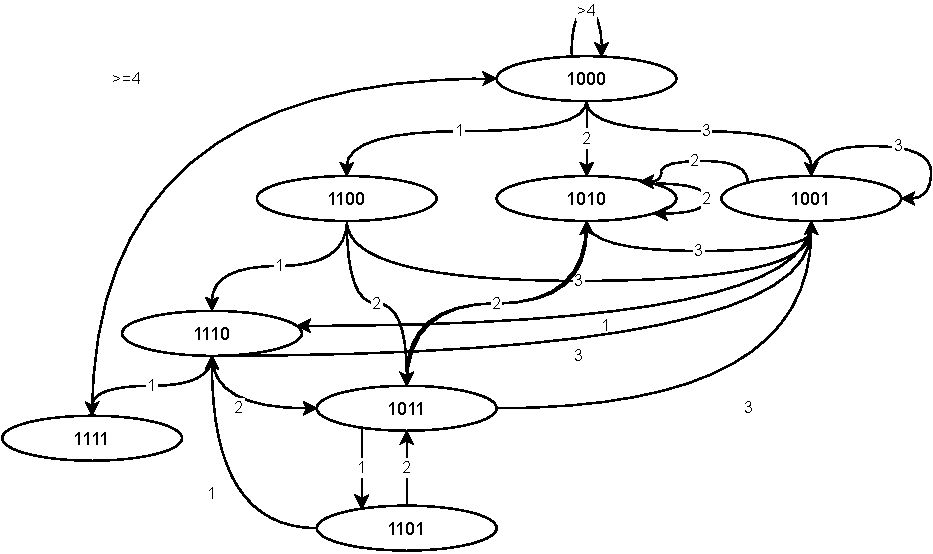
\includegraphics[width=0.5\textwidth]{4-img.pdf}
 
\end{outline}

\end{document}
